\newcommand{\walletcollector}{\texttt{wallet\_collector}}
\newcommand{\userinforetriever}{\texttt{user\_info\_retriever}}
\newcommand{\addresschecker}{\texttt{address\_checker}}
\newcommand{\graph}{\texttt{graph}}

\section{Nduja} \label{nduja}
\subsection{High level architecture}
Nduja was developed in Python\footnote{It should be used with Python3.5+} and it
is composed by four main modules, represented in Figure\ref{fig:architecture}:
\begin{enumerate*}[label=\roman*),itemjoin={,\quad}]
\item \walletcollector{} is a set of classes whose aim is to retrieve
addresses of different cryptocurrencies. It provides a different class for each
different source used, following the exact same interface
\item \userinforetriever{} is a set of classes that, based on which
site a wallet is discovered, retrieve some information (e.g. name, email,
personal website) related to the owner of that wallet
\item \addresschecker{} checks whether the recognized addresses are valid and if
they are involved at least in one transaction or not. For certain
altcoins it is not possible to perform this validation accurately, e.g.
Monero has private transactions, so it is not possible to find out that
information
\item \graph{} is the module responsible for analyzing the transaction graph
in order to retrieve the clusters.
%for create graph with which is
% possible to correlate addresses and plot graphs.
\end{enumerate*}

\begin{figure}
\centering
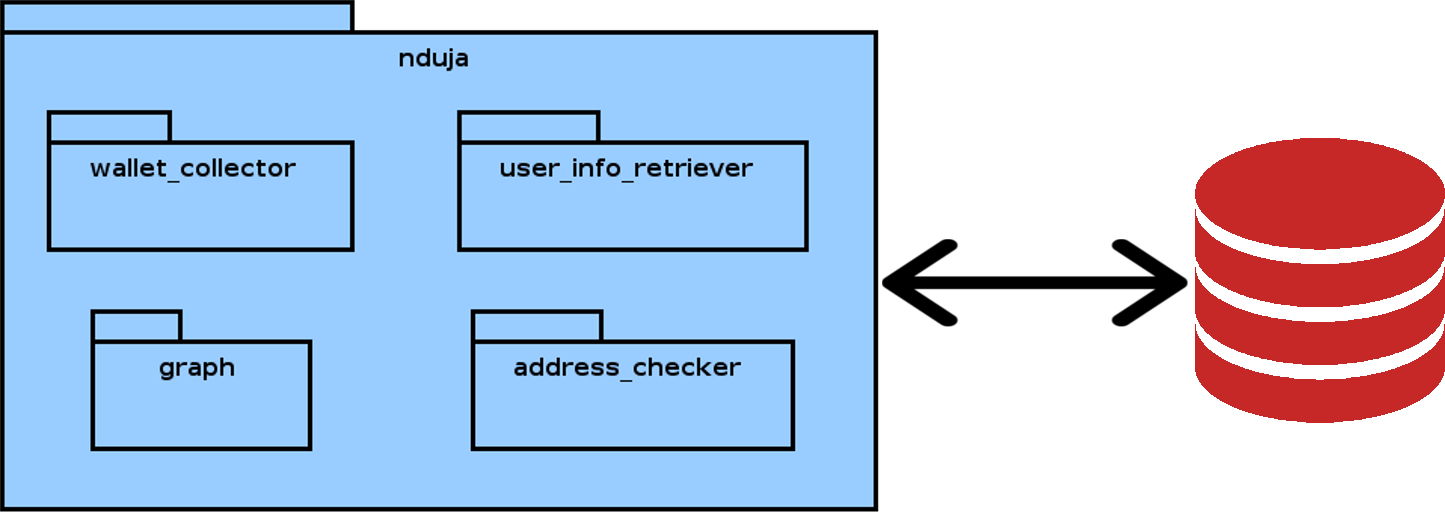
\includegraphics[width=\columnwidth]{db}
\caption{Nduja high level architecture}
\label{fig:architecture}
\end{figure}

\subsection{Queries}
\label{sec:queries}
In order to maximize the number of possible results in repositories the module
\walletcollector{} searches for files that contain words such as
\textbf{donation} or \textbf{contribution} and in which there is a set of
characters that matches the provided regular expressions defined for the
different address formats. This has been implemented using two different APIs:
Github Search API \footnote{\url{https://developer.github.com/v3/search/}} and
Searchcode API \footnote{\url{https://searchcode.com/api/}}.
In addition to the keywords searched in Github, in Twitter we searched also for
\textit{hashtags} such as \textbf{\#GiveAway} and
hashtags correlated to specific cryptocurrency (e.g. \#BTCGiveAway). This has
been done using Twitter API
\footnote{\url{https://developer.twitter.com/en/docs/api-reference-index}}.
However, it has a strong limitation: we are only able to retrieve tweets that
were published at most a week before the search. This limitation is imposed
because we have not paid for a premium account. In fact our research must be
thought as a proof of concept.
Although this limitation even with a free account one can collect a huge amount
of data by performing those queries weekly:
the information before the first search is lost without a premium account, but,
following this idea it is possible to collect incrementally all the future
addresses.

\subsection{Database}
All data retrieved is stored into a
SQLite\footnote{\url{https://www.sqlite.org/}} database. Addresses are stored
with the indication that if they are wallets retrieved from the websites we
search, if they are inferred or they are ``tagged'' addresses. These are
wallets that are known \emph{a priori}, i.e. that are used by well-known
services, such as mixing services or betting games as
\textit{SatoshiDICE}\footnote{\url{satoshidice.com}}.
The reason to exclude this kind of addresses is twofold: the former is that we
do not want that the number of addresses in the clustering phase explodes for
both time and storage constraints and the latter is that these
addresses are already ``public'', so they are useless for the sake of our study.

\subsection{Algorithm}
\texttt{Nduja} algorithm follows a sequence of 3 steps:
\subsubsection*{Data retrieving} Firstly all possible wallets are collected
and inserted into the database. In order to do this the research on
Twitter, Github and using Searchcode API is performed. The addresses
discovered are stored in relation to the account that advertised them.
In this paper we refer to \textit{Account} when we talk about a Twitter, Github
or some other repositories host profile, instead with the word \textit{Address}
or \textit{Wallet} we mean the public key of a wallet of a certain
cryptocurrency.
\subsubsection*{Account data retrieving} The second step involves the
retrieving of all possible data related to accounts inserted into the database
in the previous step. This is done by using related APIs
(e.g. Twitter API, Github Search API, Bitbucket API, etc.) to fetch the public
information of the accounts and also by searching for emails and websites in
the same resources where we found in the first place the addresses.

\subsubsection*{Clustering addresses} The last step consists in grouping
wallets that could be associated with the same person. In order to do so we
take advantage of
Blockchain.info API\footnote{\url{https://blockchain.info/api}},
Chain.so API\footnote{\url{https://chain.so/api}} and
Etherscan API\footnote{\url{https://etherscan.io/apis}}. These APIs allow
developers to query Bitcoin's, Ethereum's, Litecoin's and Dogecoin's
blockchains without having a local copy of them, that can count
hundreds of gigabytes~\cite{bib:bitinfochart}. We used the APIs to find out all
the transactions regarding a single wallet in our database.
Afterward we looked for transactions with multiple inputs that
involve wallets that we connected to a certain person to create a
``cluster'' of wallet of the same user.
